\section{Auswertung}
\label{sec:Auswertung}

% \begin{figure}
%   \centering
%   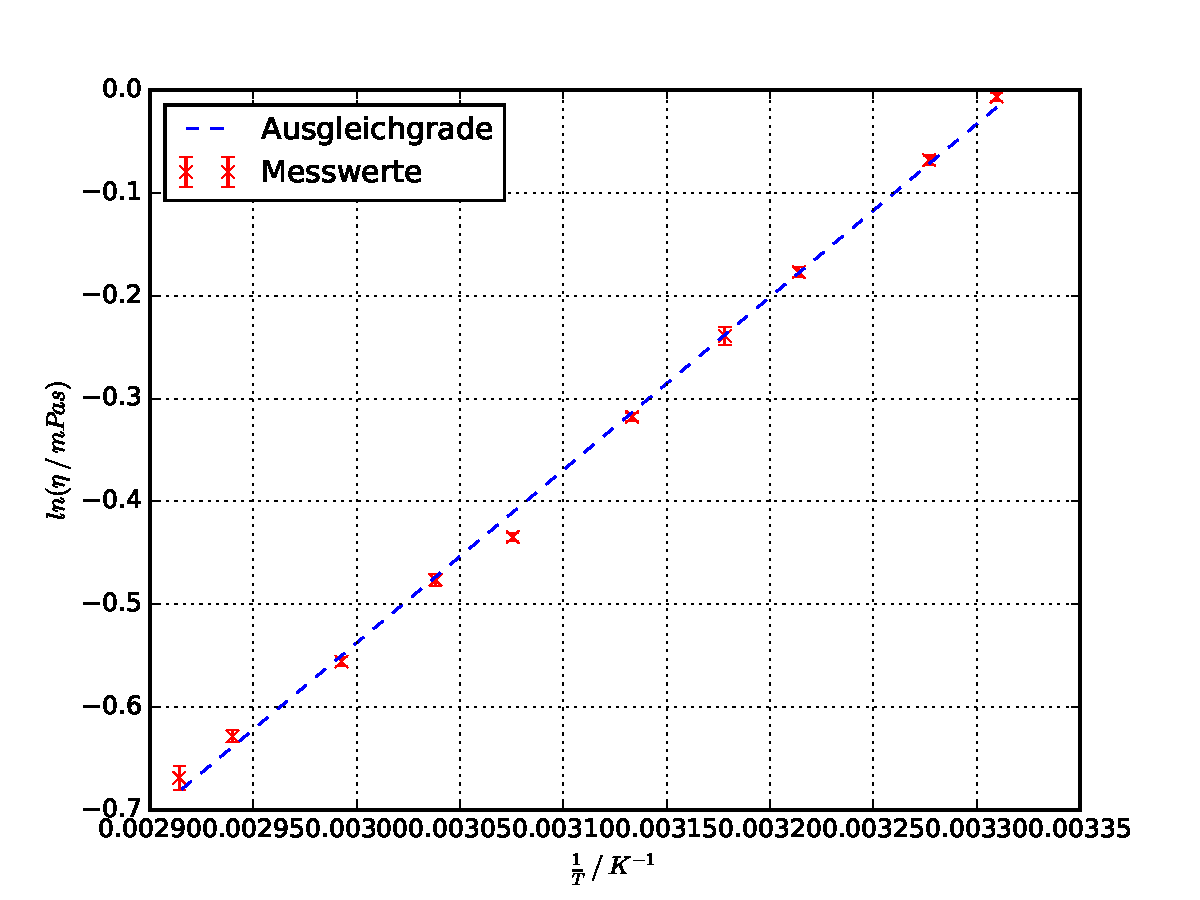
\includegraphics{plot.pdf}
%   \caption{Plot.}
%   \label{fig:plot}
% \end{figure}

\subsection{Methoden}
Alle Mittelwerte und deren Fehler wurden mit der Formel
\begin{equation}
  \langle x \rangle = \frac{1}{n} \sum_{i=1} ^{n} x_i \quad \text{und} \quad
  \Delta x = \sqrt{\frac{1}{n(n-1)} \sum_{i=1}^n (x_i - \langle x \rangle )^2}
  \label{eqn:MW}
\end{equation}
berechnet \cite{Tipler}.
\subsection{Dampfdruck und die mittlere freie Weglänge}
In der Tabelle \ref{tab:ue} sind die Temperturen, Dampfdrücke, mittlere Weglängen
sowie der Größenfaktor $ \sfrac{a}{\bar{w}}$, wobei $a = 1 \si{\centi \meter}$ bei
der verwendeten Versuchapparatur beträgt. Die Tabelle zeigt die Werte zweilenweise für
die verschieden Versuchsteile, d.h. die ersten beiden Zeilen zeigen die Werte für
die Messung der integralen Energieverteilung bei verschiedenen Temperturen, die Dritte
für die Messung der Franck-Hertz-Kurve und die vierte für die Messung de Ionisierungsspannung.
Der Größenfaktor sollte zischen 1000 und
4000 liegen, da sonst keine ausreichend große Stoßwahrscheinlichkeit gewährleistet ist.
Aus der Tabelle \ref{tab:ue} ist also zu entnehmen, dass nur bei der Messung
der integrale Energieverteilung eine ausreichende
Stoßwahrscheinlichkeit gewährleitstet war.

\begin{table}
  \centering
  \caption{Temperaturen, Dampfdrücke , mittlere freie Weglängen und Größenfaktor von
  \texorpdfstring{$a$}{math} und \texorpdfstring{$\bar{w}$}{math} im Überlick }
  \sisetup{ round-mode = places, round-precision = 2 ,table-format = +3.2e+2}
  \begin{tabular}{S[scientific-notation = fixed , fixed-exponent = 0] S S S[scientific-notation = fixed , fixed-exponent = 0]}
    \toprule
    $T$ / \si{\kelvin} & $p_{sät}$ / \si{\milli \bar} & $\bar{w}$ / \si{\centi \meter} & $\frac{a}{\bar{w}} $ \\
    \midrule
    2.963499999999999659e+02 & 4.610353052222010764e-03 & 6.290190723251254390e-01 & 1.589776914559314136e+00\\
    4.321499999999999773e+02 & 6.764590844732246921e+00 & 4.287029425080899009e-04 & 2.332617532666292391e+03\\
    4.711499999999999773e+02 & 2.524846657539852046e+01 & 1.148584604668898143e-04 & 8.706367784620180828e+03\\
    3.761499999999999773e+02 & 6.331184373651318475e-01 & 4.580501575769957597e-03 & 2.183167025397006569e+02\\
    \bottomrule
  \end{tabular}
  \label{tab:ue}
\end{table}
\subsection{Differentielle Energieverteilung}
\begin{landscape}
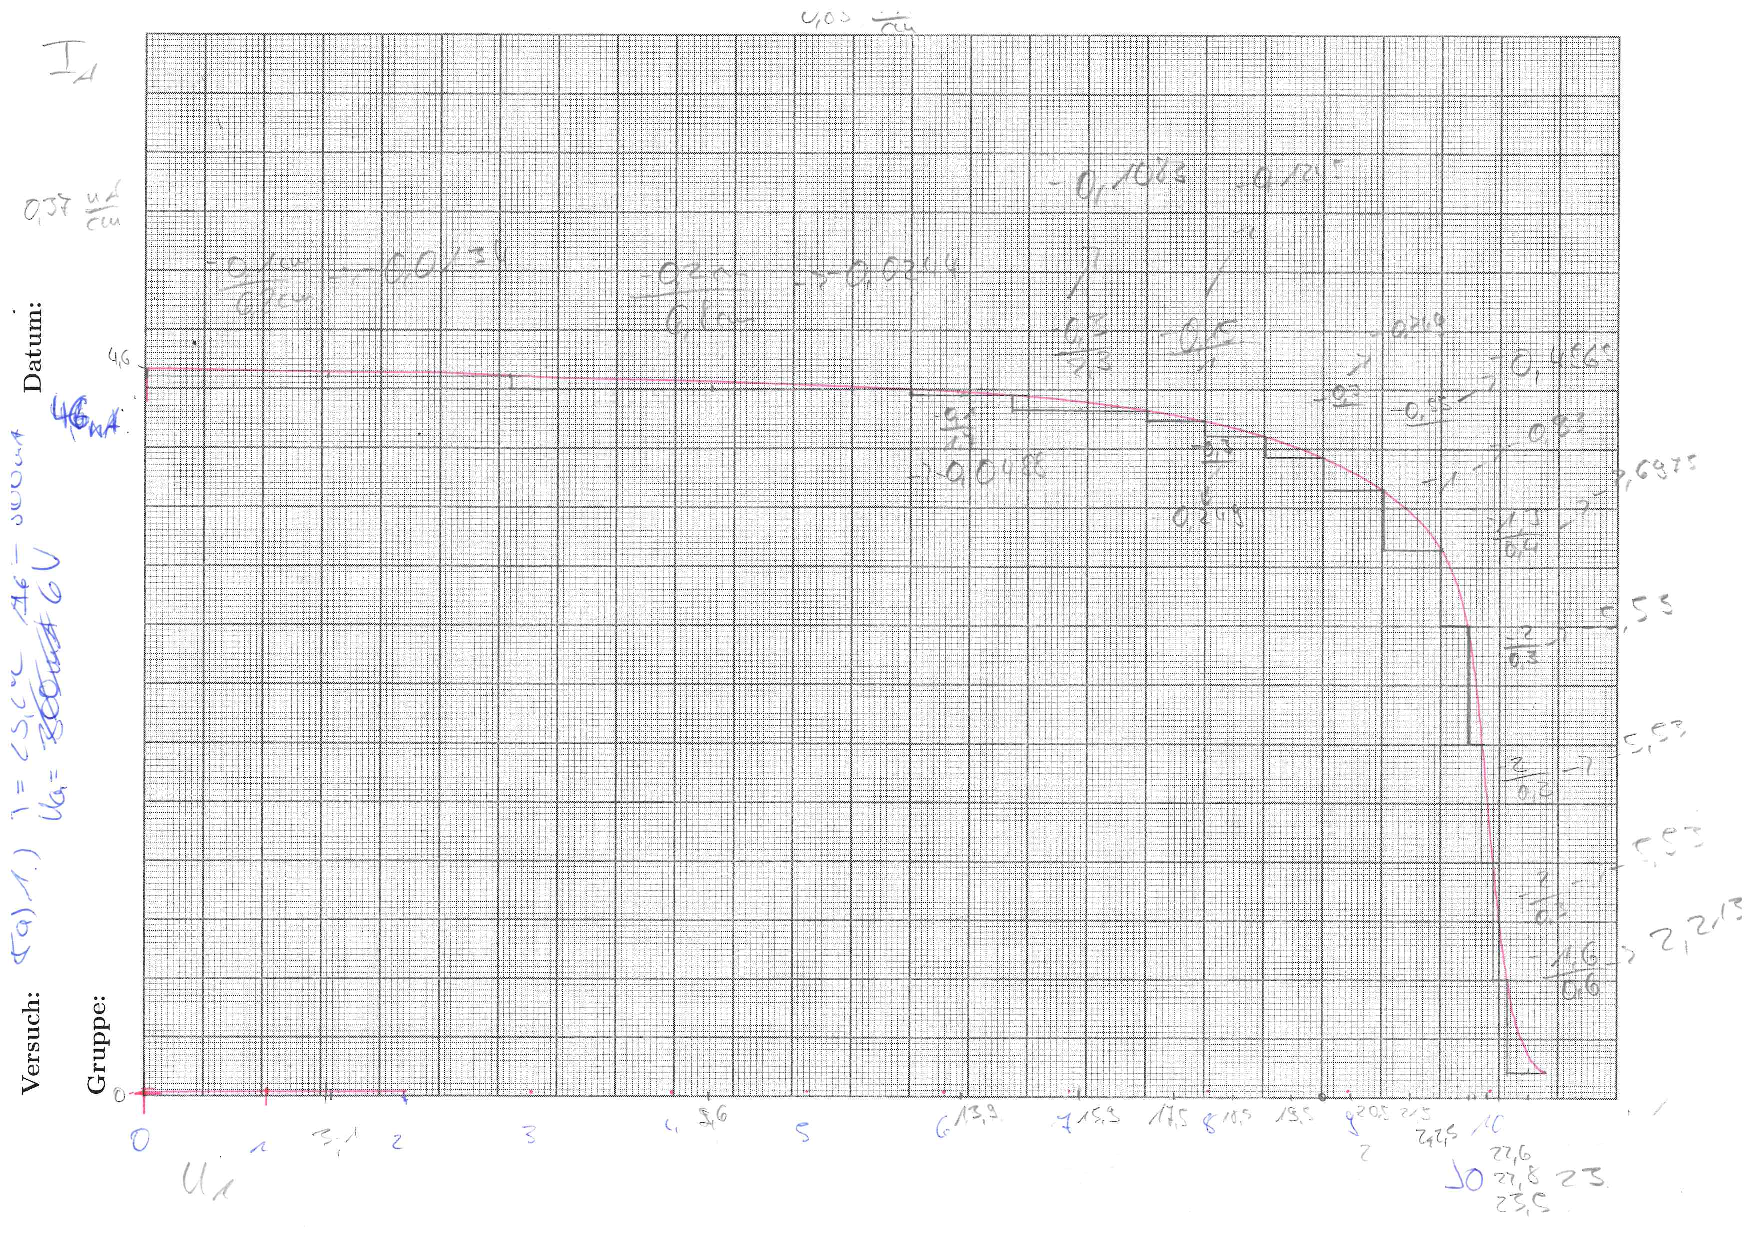
\includegraphics[page = 1, scale = 0.8]{8a1.pdf}
\label{fig:8a1}
\end{landscape}
\begin{landscape}
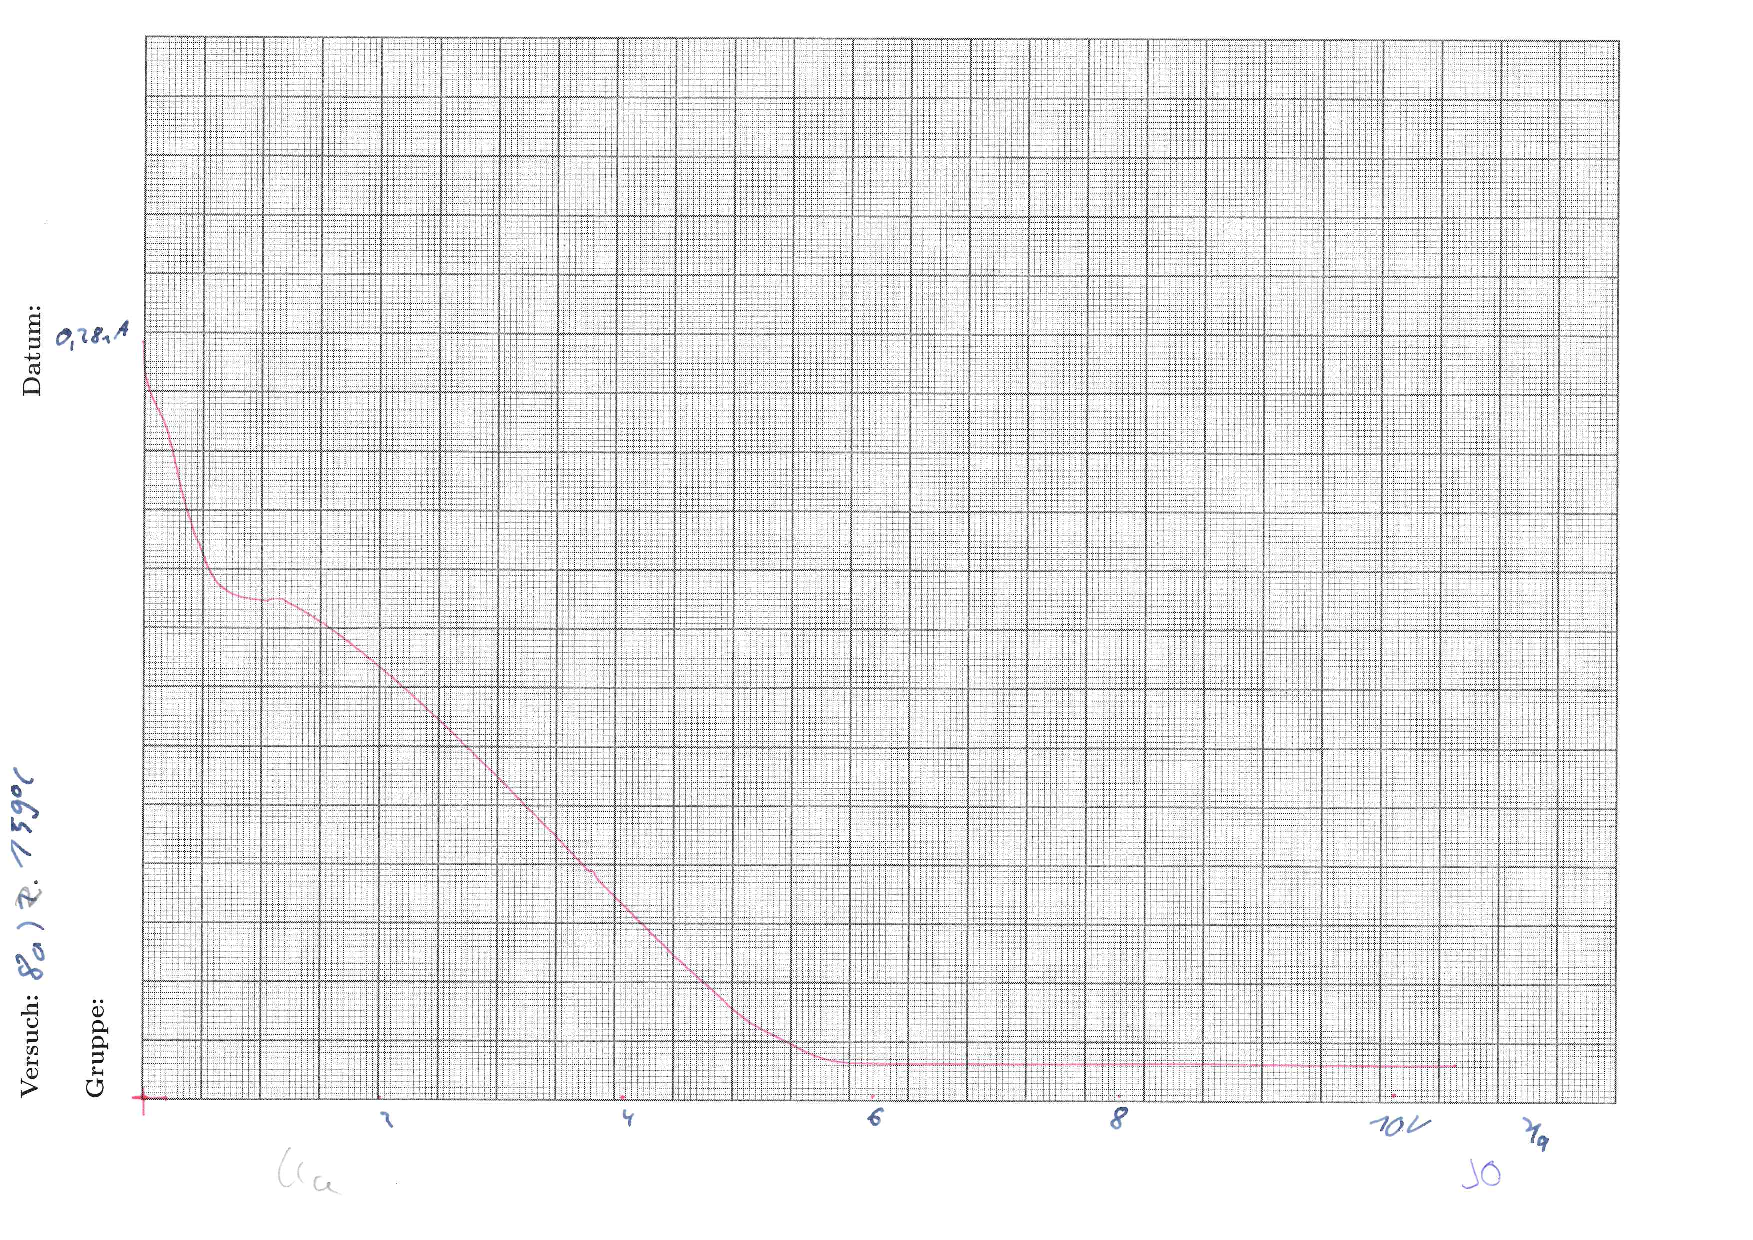
\includegraphics[page = 1, scale = 0.8]{8a2.pdf}
\label{fig:8a2}
\end{landscape}
\subsection{Franck-Hertz Kurve}
\begin{landscape}
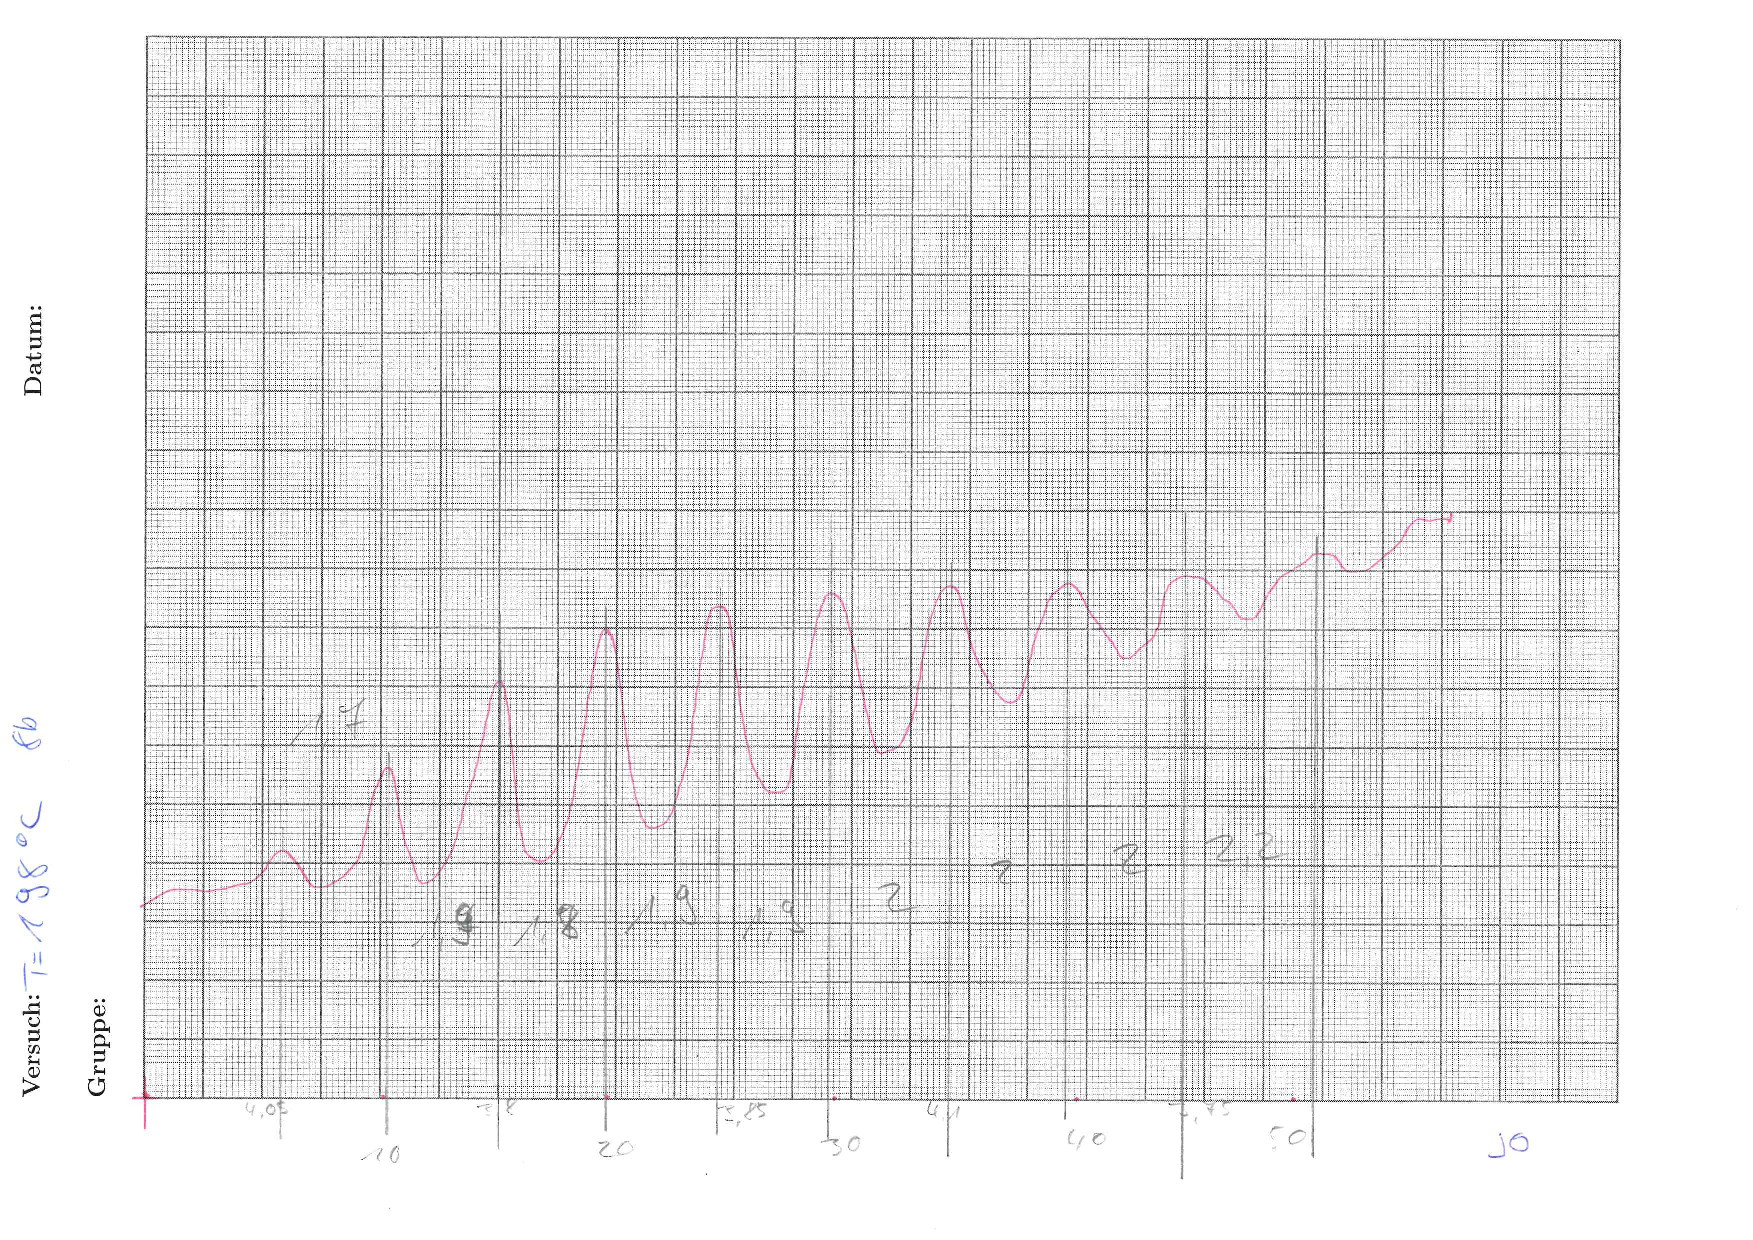
\includegraphics[page = 1, scale = 0.8]{8b.pdf}
\label{fig:8b}
\end{landscape}
\subsection{Ionisierung}
\begin{landscape}
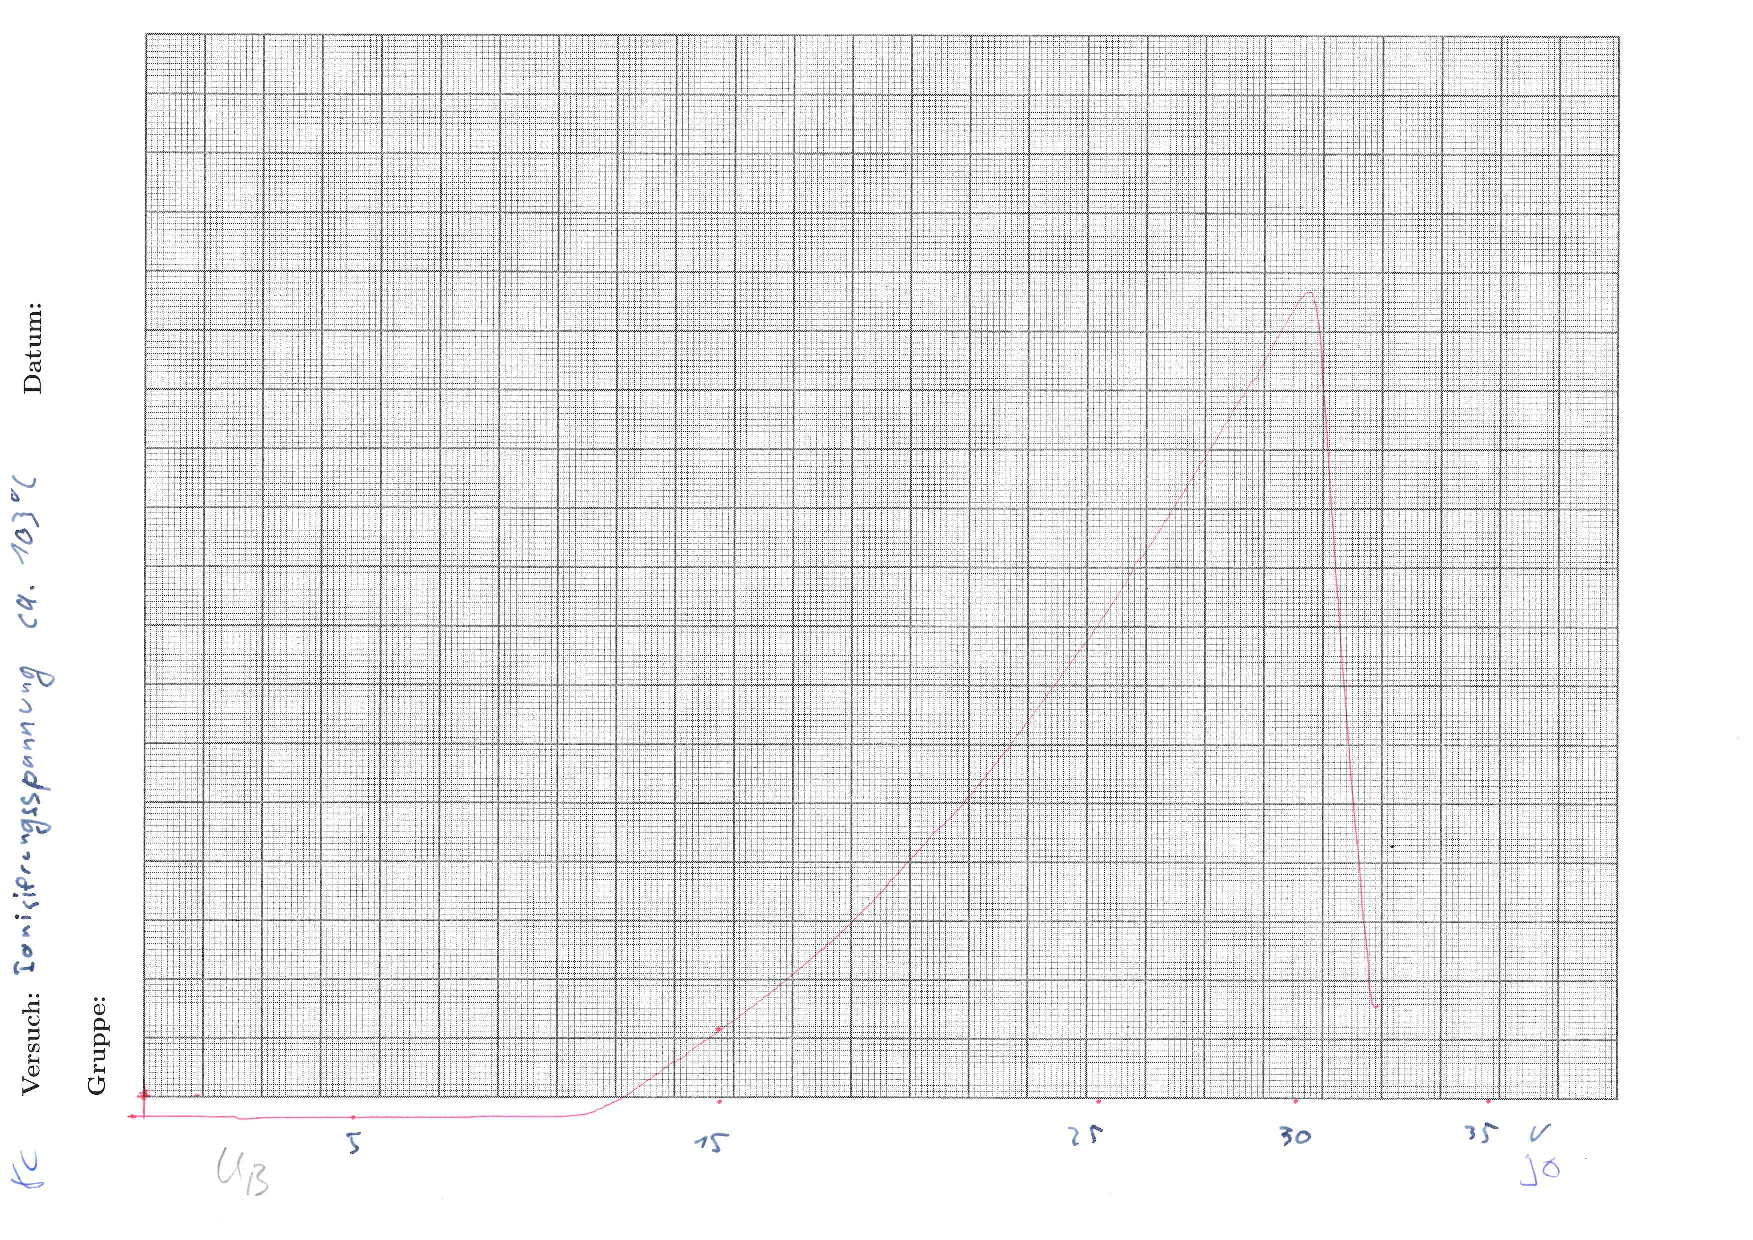
\includegraphics[page = 1, scale = 0.8]{8c.pdf}
\label{fig:8c}
\end{landscape}
